\documentclass[a4j,twocolumn]{jsarticle}

\usepackage[dvipdfmx]{graphicx}

\setlength{\textheight}{275mm}
\headheight 5mm
\topmargin -30mm
\textwidth 185mm
\oddsidemargin -15mm
\evensidemargin -15mm
\pagestyle{empty}

\begin{document}
\title{Mg-LPSO の Small Cluster の第一原理計算}
\author{情報科学科 西谷研究室 3539 山本 泰基}
\date{}
\maketitle


\section{背景}
\vspace{-0.5em}
LPSO(Long Period Stacking Order)構造をもった Mg は比降伏強度で超々ジュラルミンの 1.2 倍の特性を持ち, かつ難燃性であるため次世代の航空機の構造材料として国内外から注目を集めている\cite{Th}. LPSO 構造は, 母相 hcp 構造の [0001] 方向に対して周期的に積層欠陥が導入されることで長周期性を有する構造である.

西谷研究室では, この LPSO 構造の生成機構として「積層欠陥部に L1$_2$ クラスターが形成され, そこから排斥された Zn, Y が, 濃化して新たな L1$_2$ クラスターを形成する」というシナリオを立て,その実現性を第一原理計算を用いて評価してきた. 計算の結果, 系全体のエネルギーは溶質原子と L1$_2$ クラスターとの距離が離れるにつれ単調に減少した. しかし,それは中周期的に溶質原子が規則化するという LPSO の構造から予想される結果に反するものであった.

本研究では, 「Small Cluster と L1$_2$ クラスターの相互作用」および「空孔を含んだクラスターの安定性」に関して第一原理計算をおこなった.

\section{手法}
\vspace{-0.5em}
本研究では初めに, Small Cluster と L1$_2$ クラスターの相互作用を調べるため, 図\ref{slab} に示す 18層の slab モデルで計算をおこなった. L1$_2$ クラスターから [0001] 方向に 1層ずつ離した位置に Small Cluster を挿入し, VASP を用いて第一原理計算をおこない, 構造緩和したエネルギーを求めた.しかし, 18層では Small Cluster と L1$_2$ クラスターの距離を 8層以上離した計算ができなかった. そこで, 18層の slab モデルを [0001] 方向に拡張した 24層の slab モデルを構築し, 同様にして計算をおこなった.

空孔とクラスターを含んだ Mg 結晶の安定性を検証するために, Small Cluster の周りに空孔を配置した. 図\ref{vacancy} で表したように, 空孔を [0001] 方向に Small Cluster の (a) 真下, (b) 真上, (c) バルク中 の位置に挿入した. 

\begin{figure}[htbp]
    \begin{tabular}{cc}
      \begin{minipage}{0.4\hsize}
        \centering
        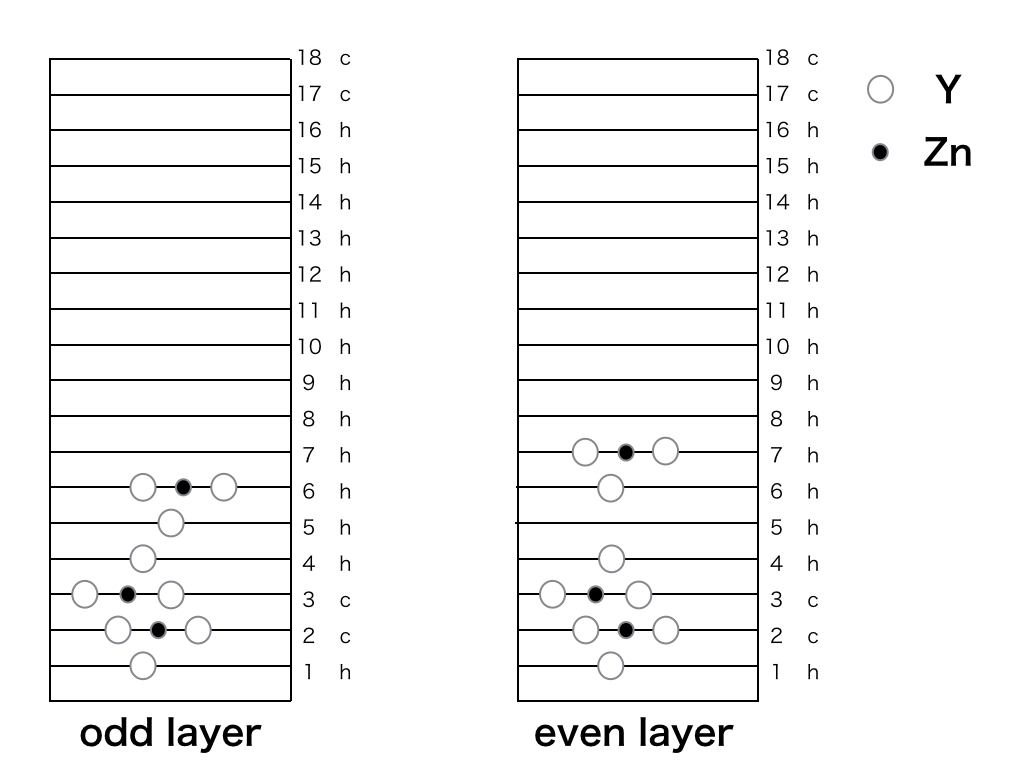
\includegraphics[width=45mm]{small_cluster_slab18.png}
		\caption{slab モデルの模式図.}
		\label{slab}
      \end{minipage} &
      \begin{minipage}{0.4\hsize}
        \centering
        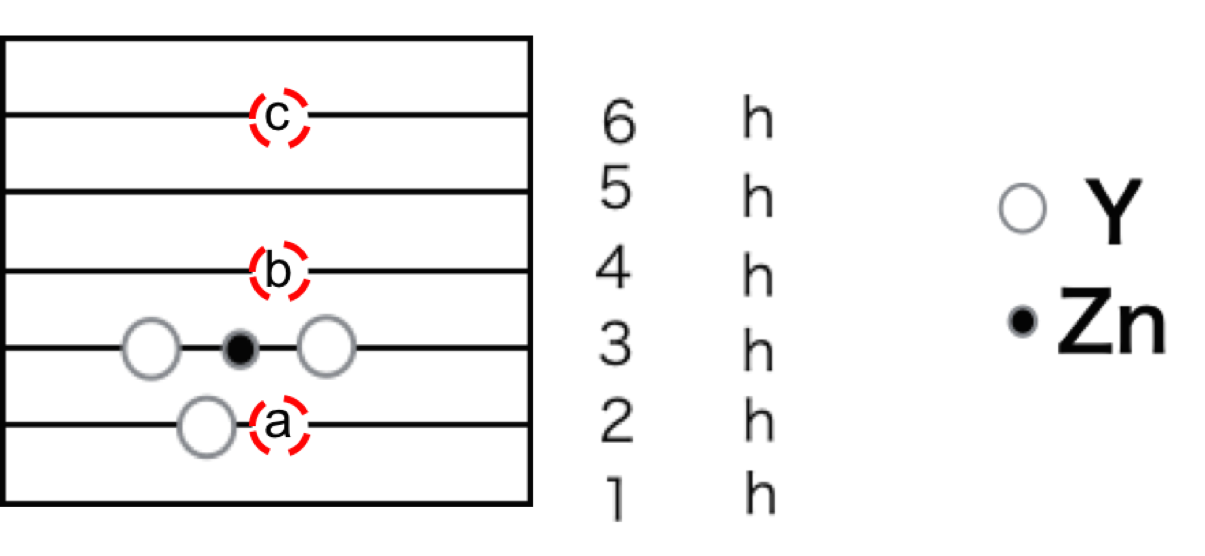
\includegraphics[width=45mm]{vacancyposition.png}
		\caption{空孔の挿入位置の模式図.}
		\label{vacancy}
      \end{minipage}
    \end{tabular}
    \vspace{-2em}
  \end{figure}
\section{考察}
\vspace{-0.5em}

18層と 24層の slab モデルについての計算結果を図\ref{fig4.1}に示す. 赤線は 24層の slab モデルのエネルギー, 緑線は 18層の slab モデルのエネルギーを示している. また, 左側の x 軸は 24層のエネルギー, 右側は 18層のエネルギーを表している. 18 層の計算では, 4 層の計算が収束しなかった. また, 8 層以降では周期的境界条件より反対側のクラスターとの相互作用が現れ, 検証する事ができなかった. そこで, 24層の slab モデルでの計算を行う事により, 4 層でも計算値が収束し, 最もエネルギーが安定するという結果が得られた.これは溶質原子が積層欠陥部から中距離離れた位置で安定化するシナリオを支持する結果となった. また, 8 層以降の層のエネルギー傾向は単調増加が止まり, 離した先にある別の L1$_2$ クラスターから影響を受けないという事が確認された.


\begin{figure}[htbp]
\begin{center}
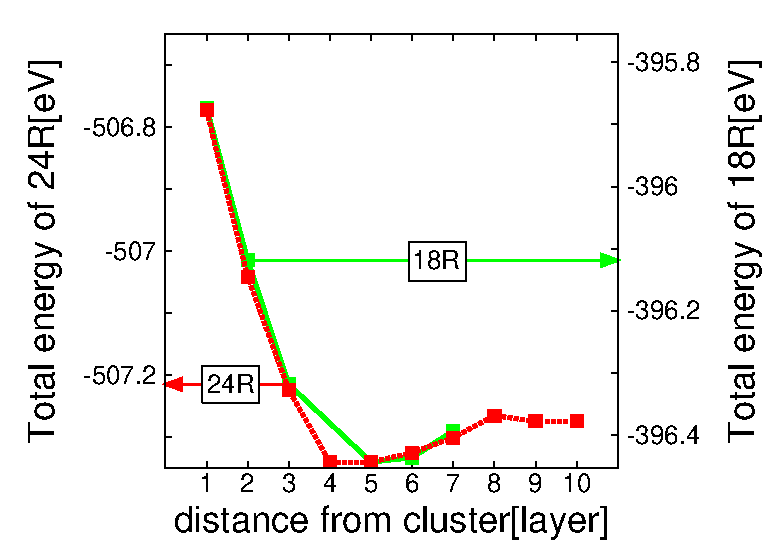
\includegraphics[width=55mm]{smallcluster_18_24.eps}
\caption{L1$_2$ クラスターと small cluster の距離によるエネルギー変化.}
\label{fig4.1}
\end{center}
    \vspace{-2em}
\end{figure}

表1は空孔を挿入したモデルの系全体のエネルギーを表している.今回の計算結果では Small Cluster から 3 層離した位置に空孔を挿入したモデルが最安定であった. これは, Small Cluster の周りに空孔が吸着し, クラスター拡散が誘発されるという当初の仮説に反するものであった. 

\begin{table}[htb]
\caption{空孔を挿入した系全体のエネルギー.}
  \begin{center}
  \small
    \begin{tabular}{lc} \hline
 挿入位置 & エネルギー [eV] \\ \hline
   (a) 真下 & -268.45\\
   (b) 真上 & -267.93\\
   (c) バルク中 & -268.50\\
\hline
    \end{tabular}
  \end{center}
  \vspace{-0.5em}
\end{table}

今後,他のサイトについても計算を行い,クラスター拡散の可能性を検証する必要がある.

\begin{thebibliography}{9}
\bibitem{Th}Y. Kawamura, K. Hayashi, A. Inoue and T. Masumoto: Mater. Trans., {\bf 42} (2001), 1172.

\end{thebibliography}


\end{document}